\documentclass{beamer}
\usepackage{graphicx}
\usepackage{xcolor}

\title{Fighting the Enemy Within}
\subtitle{Basic Life Science and Issues : Presentation}
\author{Group 4}
\institute{Chungnam National University}
\date{November, 2019}

\usetheme{metropolis}

\beamertemplatenavigationsymbolsempty
\setbeamertemplate{footline}{%
    \hspace{1em}%
    
\includegraphics[height=3em]{0}
    \hfill%
    \usebeamerfont{footline}%
    \usebeamercolor[fg]{footline}%
    \hspace{1em}%
    Fighting the Enemy Within \hspace{1em} %
    \insertframenumber/\inserttotalframenumber%
    \hspace{1em}%
    \vspace{1em}%
}

\begin{document}
    \begin{frame}[plain]{ }
        \maketitle
    \end{frame}

    \begin{frame}{Group Members}
        \begin{itemize}
            \item \textbf{Chaeeun Kim}

                  College of Medicine, 19'
            \item \textbf{Jongkwan Bae} 
            
                  Dept of EE Comm. Engineering Education, 17'
            \item \textbf{Seungmin Lee}
            
                  College of Medicine, 19'
            \item \textbf{Kangjun Heo}
            
                  Dept of Computer Science and Engineering, 17'
        \end{itemize}
    \end{frame}

    \begin{frame}{Chapter Abstraction}
        \textbf{Fighting the Enemy Within}
        
        11th chapter of \textit{The Epigenetics Revolution}

        \vspace{2.5em}

        \textit{"Epigenetic perspective of Cancer and its treatment"}
    \end{frame}

    \begin{frame}{Introduction: Cancer}
        Healthy cells, have two types of genes:
        \begin{itemize}
            \item proto-oncogenes for cell proliferation
            \item tumor suppressor genes for regulation
        \end{itemize}
    \end{frame}

    \begin{frame}{Introduction: Cancer}
        Healthy cells, have two types of genes:
        \begin{itemize}
            \item proto-oncogenes for cell proliferation
            \item tumor suppressor genes for regulation
        \end{itemize}

        However, cancer cells lost balance of these, For example,
        \begin{itemize}
            \item proto-oncogenes is over-activated
            \item tumor suppressor genes is inactivated
        \end{itemize}
    \end{frame}

    \begin{frame}{Introduction: Cancer}
        Healthy cells, have two types of genes:
        \begin{itemize}
            \item proto-oncogenes for cell proliferation
            \item tumor suppressor genes for regulation
        \end{itemize}

        However, cancer cells lost balance of these, For example,
        \begin{itemize}
            \item proto-oncogenes is over-activated
            \item \textcolor{red}{tumor suppressor genes is inactivated}
        \end{itemize}
    \end{frame}

    \begin{frame}{Epigenetic Approach for Oncogenesis}
        \begin{itemize}
            \item DNA Methylation
            
                  \vspace{1em}
                  Hypermethylation of CpG island

            \vspace{3em}
            \item Repressive Histone Modification
                  
                  \vspace{1em}
                  Histone deacetylation
        \end{itemize}
    \end{frame}

    \begin{frame}{DNA Methylation}
        Cytosine before Guanine can be methylated

        \begin{center}
            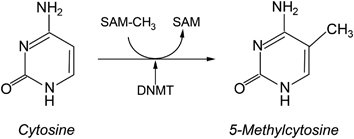
\includegraphics{5mc.png}
        \end{center}

        Methyl group is bond on 5' carbon atom
    \end{frame}

    \begin{frame}{DNA Methylation}
        CpG dinuclotide cluster (CpG island, CGI) are usually located in the promoter regions of genes in a DNA sequence.
        \begin{center}
            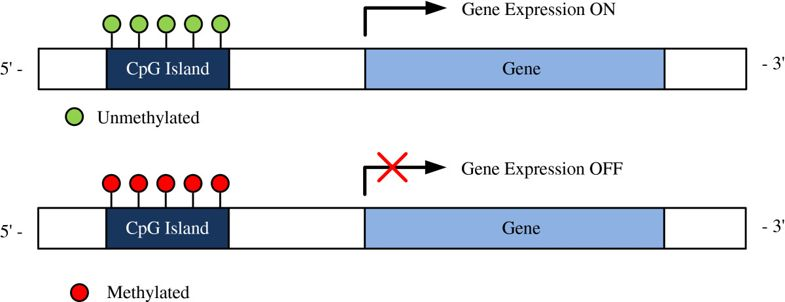
\includegraphics[height=8em]{1}
        \end{center}
        Hypermethylated CGI disables specific gene expression.
    \end{frame}

    \begin{frame}{Histone deacetylation}

    \end{frame}

    \begin{frame}{Characteristics of Oncogenesis}
        \begin{itemize}
            \item Multi-step process
            \item Defections must be accumulated
                  
                  \vspace{1em}
                  {\small Inherited oncogenes are slowly expressed 
                  
                  e.g.) BRCA1 mutation}
                  \vspace{1em}

            \item Tumour suppressor gene alteration - Switched off
            \item Epigenetical access
        \end{itemize}
    \end{frame}

    \begin{frame}{Approach for Treatment}
        \begin{itemize}
            \item DNMT enzyme inhibitors
            
                  {\small 5-azacytidine, 2-aza-5’-deoxycytidine}
                  
                  \vspace{2em}
                  \begin{center}
                    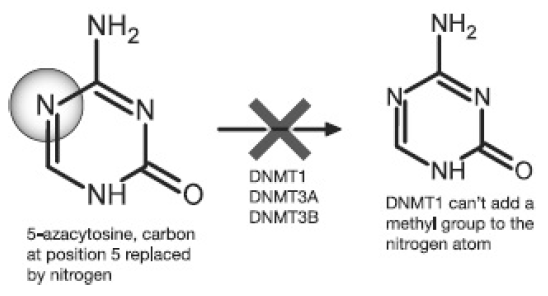
\includegraphics[height=6em]{5azcy-inh}
                    
                    {\footnotesize methylation inhibited by 5-azacytidine}
                  \end{center}
        \end{itemize}

    \end{frame}

    \begin{frame}{No easy wins}

    \end{frame}

    \begin{frame}{Alternative Approach}

    \end{frame}

    \begin{frame}{Conclusion}

    \end{frame}

    \begin{frame}{References}
        \footnotesize [1] Carey, N. (2012). \textit{The Epigenetics Revolution}. Columbia University Press
    
        \footnotesize [2] Kakumani, R.; et al. (2012). \textit{Identification of CpG islands in DNA sequences using statistically optimal null filters}, EURASIP Journal on Bioinformatics and Systems Biology 
    
        \footnotesize [3] Kazantsev, Aleksey G; et al. (2008). \textit{Therapeutic application of histone deacetylase inhibitors for central nervous system disorders}, Nature Reviews. Drug Discovery\; London Vol. 7 Iss. 10\: 854-68.
    \end{frame}

    \begin{frame}[plain]
        \centering
        \huge Q \& A
    \end{frame}

    \begin{frame}[plain]
        \centering
        \huge Thank you!
    \end{frame}
\end{document}